\subsubsection{Kubuntu 16.04}

Am Host-PC muss bei den IPv4-Einstellungen auf Methode "`Automatisch"' eingestellt sein. Wenn es sich um eine neue Verbindung handelt ist dies bereits voreingestellt und eine Parametrieren kann entfallen. Ansonsten
muss zur Konfiguration unter Linux (Kubuntu 16.04) zuerst "`Netzwerkverbindungen"' ge�ffnet werden.\\ 
Dazu klickt man mit der rechten Maustaste auf das Netzwerksymbol in Infobereich rechts unten. Dann kann die Option "`Netzwerkverbindungen einrichten..."' ausgew�hlt werden.

\begin{figure}[ht]
  \centering
  
\includegraphics[scale=1.00]{images/OTG_NetzwerkverbindungenIcon.png}	
  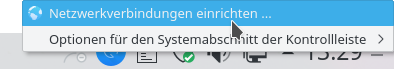
\includegraphics[scale=0.42]{images/OTG_NetzwerkverbindungenOpen.png}	
  %	\caption{}
  \label{OTG_LINUX_NetzwerkverbindungenApp}
\end{figure}


Dann kann die neue "`Kabelnetzwerkverbindung"' umbenannt werden, z.~B. in Raspberry Pi Zero. Erkennen kann man das Netzwerk an der Mac-Adresse die man bei "`g\_ether.host\_addr"' angegeben hat (z.~B. 00:01:02:03:04:05).  


\begin{figure}[ht]
  \centering
  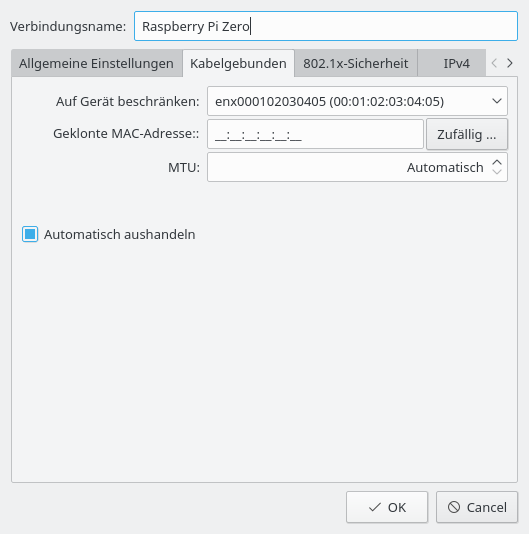
\includegraphics[scale=0.42]{images/OTG_Pi_Verbindungsname.png}
	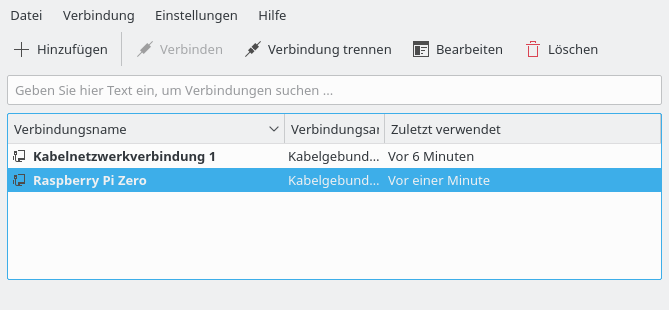
\includegraphics[scale=0.42]{images/OTG_Netzwerkverbindungen.png}
%	\caption{}
  \label{OTG_LINUX_Netzwerkverbindungen}
\end{figure}


Nun kann bei den IPv4-Einstellungen auf Methode "`Automatisch"' eingestellt werden.

%\begin{figure}[ht]
%  \centering
%  \includegraphics[scale=0.42]{images/OTG_NetzwerkverbindungenAutomatisch.png}
%	\caption{}
%  \label{OTG_LINUX_Netzwerkverbindungen}
%\end{figure}

%\subsection{Internet Zugriff} 
~\\
Nach der Einrichtung des Netzwerk kann der Raspberry Pi Zero mit dem Namen "`raspberrypi.local"' erreicht werden. Um den Raspbery Pi Zero mit dem Internet verbinden zu k�nnen m�ssen einige Einstellungen am Host %und Client
 gemacht werden. Man muss den Name des Netzwerkger�ts am Host-PC kennen, das mit dem Internet verbunden ist. Dies ermittelt man �ber die Netzwerkeinstellungen oder �ber die Konsole mit nmcli. Im Beispielfall ist der Name "`enp0s25"' das richtige Ger�t.

\begin{console} 
	nmcli d
\end{console} 

\begin{screensmall} 
	GER�T            TYP       STATUS           VERBINDUNG        
	enx000102030405  ethernet  verbunden        Raspberry Pi Zero 
	enp0s25          ethernet  verbunden        Netzwerkverbindung 1                
	lo               loopback  nicht verwaltet  --  
\end{screensmall}

Damit der Internetzugang f�r den Raspberry Pi Zero freigegeben wird, m�ssen am Host-PC folgende Befehle in einem Terminal eingeben werden. "`enp0s25"' muss durch den Namen des Netzwerkger�ts ersetzt werden, das mit dem Internet verbunden ist.

\begin{console} 
	sudo sysctl -w net.ipv4.ip_forward=1
	sudo iptables -t nat -A POSTROUTING -o enp0s25 -j MASQUERADE
\end{console}





